\section{Sampling and Sorting}

\begin{definition}[Algorithm]
  Downald Knuth defines Alrgorithm as a \textit{finite, definite,
  effective procedure, with some output}.

  \begin{itemize}
    \item\textbf{Finite}: An algorithm must always terminate after a
      finite number of steps\dots a very finite numer, a reasonable numer.
    \item\textbf{Definite}: Each step of an algorithm must be
      precisely defined; the action to be carried out must be
      rigorously and unambiguously specified for each case.
    \item\textbf{Effective}: All of the operations to be performed
      in the algorithm must be sufficiently basic that they can in
      principle be done exactly and in a finite lenght of time by a
      man using paper and pencil.
    \item\textbf{Procedure}: The sequence of specific steps arranged
      in a logical order.
    \item\textbf{Input}: Quantities which are given to it initlially
      before the algorithm begins. These inputs are taken from
      specified sets of objects.
    \item \textbf{Output}: Quantities which have a specified relation
      to the inputs.
  \end{itemize}
\end{definition}

\subsection{Time Complexity}

Time complexity is measured over the number of steps $T(n)$, where
$n$ is the input size. We take the maximum $T(n)$ over
all the inputs that induce in the worst behavior and we call it
\textit{worst case}.

\subsection{The RAM model}

\begin{figure}[h!]
  \centering
  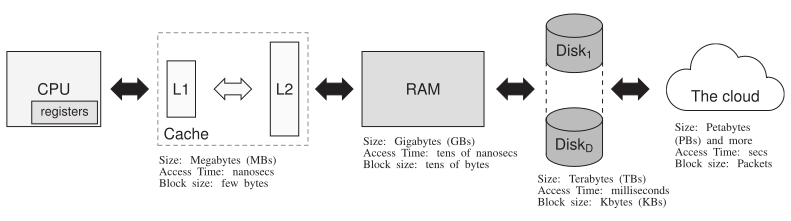
\includegraphics[width=1\textwidth]{images/memory_levels.png}
  \caption{Memory Access Levels and the access Time}
  \label{fig:memory_access_levels}
\end{figure}

\textit{Random Access Memory} model is a type of computing model
where the memory size is assumed to be infinite, so every operation
done on the \texttt{CPU} is assumed to be a finite value. This can lead
out the importance of memory access, where as shown in
Figures~\ref{fig:memory_access_levels}, if not handled correctly can
drasticly reduce the efficiency of our
algorithms due to the \textit{time} needed to fetch new data from
different levels of memory which can increase drasticly.
If we try to read a value bigger than the capacity of our registers
that can lead to use more than one \texttt{IOs} operation to execute
a computational step which we assumed as one in the \textbf{RAM} model.

\subsection{Why should we care about Asymthotics}

Here we are gona show how the importance of algorithm complexity if
much important than the speed of our machine by using this three examples.

\[
  \begin{cases}
    T_1(n) = n  \rightarrow n = t \rightarrow n^{'} = k \times t \\

    T_2(n) = n^2 \rightarrow n = \sqrt{t} \rightarrow n^{'} = \sqrt{k
    \times t} \\

    T_3(n) = 2^n \rightarrow n = \log_{2}{t} \rightarrow n^{'} =
    \log_{2}{k} + \log_{2}{t}\\
  \end{cases}
\]

Here $k$ rappresent a faster machine, as the complexity
of the algorithm from $T_1$ to $T_3$ increase we can see that even if
we use a $k$ faster machine with the $T_2$ and $T_3$ algorithm the
increase in speed and efficiency is not notable.

\subsection{Summing items in an Array}

A simple algorithm on which we can do a simple \texttt{IOs}
complexity analisys can be the \textit{Sum of elements in an Array}.
We define an array as in Figures~\ref{fig:sum_of_elements_array}, and
than we \texttt{SCAN} it (we
read from left to right), block by block and sum the elements in the
block to the accumulation variable.

\begin{figure}[h!]
  \centering
  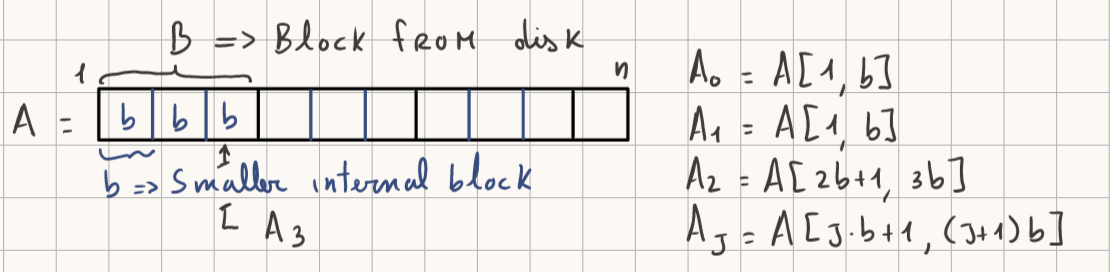
\includegraphics[width=1\textwidth]{images/sum_of_elements.png}
  \caption{Sum of elements in an array}
  \label{fig:sum_of_elements_array}
\end{figure}

In this example we rappresent memory blocks, readed from the disk, by
the $B$ label, than the sub-blocks subdivinding the $B$ in smaller
blocks as $b$, and the access to those smaller block as $A_{0 \text{ or }
1} = A[1,b]$, $A_{2} = A[2b + 1,3b]$ and than the generic $A_{j} =
A[jb + 1, (j + 1)b]$.
The number of \texttt{IOs} operation is calculated as $\#\texttt{IOs}
= \frac{n}{\#B}$.
The following algorithm shows how to sum the the elements of all the
blocks in the array.

\begin{algorithm}
  \caption{Sum of elements}
  \label{algo:sum_of_elements_array}
  \begin{algorithmic}[1] % Show numbers
    \Procedure{Sum of elements}{$A, s, n, b$}
    \State $sum \gets 0$
    \For{$i = 0$ \textbf{to} $(n/b) - 1$}
    \State $j \gets (i \times s) \bmod (n/b)$
    \State $sum \gets sum + \text{somma degli elementi in } A_j$
    \EndFor
    \State \Return $sum$
    \EndProcedure{}
  \end{algorithmic}
\end{algorithm}

The algorith iterate over $\frac{n}{b}$ times which is equal to the
total sub-blocks.
Each iteration calculates $j$ as the iteration time $(i \times s)
\mod \frac{n}{b}$ where $s$ is equal to the next step in the array.

\subsubsection{\texttt{IO} Complexity}
When $s = 1$ it scan the array jumping from $A_i \rightarrow A_{i +
1}$ but when $s > 1$ than it can jump more than
$+1$ position in the array.
We can obtain the algorith \texttt{IO} Complexity as:
$$\texttt{IO }\text{Complexity} = \frac{n}{B} \times \min\{s, \frac{B}{b}\}$$
$$s \le \frac{B}{b} \rightarrow s \times \frac{n}{B}$$
$$s > \frac{B}{b} \rightarrow \frac{n}{\cancel{B}} \times
\frac{\cancel{B}}{b} = \frac{n}{b}$$

\noindent Where $\frac{B}{b}$ rappresent the number of total possible
sub-blocks.

\subsection{Binary Search}
